\documentclass[11pt,a4paper]{article}

\usepackage[margin=2.2cm]{geometry}
\usepackage[T1]{fontenc}
\usepackage[utf8]{inputenc}
\usepackage{lmodern}
\usepackage{microtype}
\usepackage{setspace}
\usepackage{booktabs}
\usepackage{longtable}
\usepackage{array}
\usepackage{amsmath}
\usepackage{hyperref}
\usepackage{xcolor}
\usepackage{listings}
\usepackage{tikz}
\usepackage{enumitem}
\usepackage{titlesec}
\usepackage{fancyhdr}

\usetikzlibrary{positioning,arrows.meta,matrix,calc}

\hypersetup{
  colorlinks=true,
  linkcolor=black,
  urlcolor=blue!50!black,
  pdftitle={Kristallball --- Military Asset Management},
  pdfauthor={Tarandeep Singh Juneja}
}

\definecolor{codebg}{RGB}{246,246,246}
\lstset{
  basicstyle=\ttfamily\footnotesize,
  backgroundcolor=\color{codebg},
  frame=single,
  framesep=6pt,
  breaklines=true,
  columns=fullflexible,
  keepspaces=true
}

\pagestyle{fancy}
\fancyhf{}
\fancyhead[L]{\small Kristallball}
\fancyhead[R]{\small NxtWave Assessment}
\fancyfoot[C]{\thepage}
\renewcommand{\headrulewidth}{0.4pt}

\titleformat{\section}{\large\bfseries}{\thesection.}{0.6em}{}
\titleformat{\subsection}{\normalsize\bfseries}{\thesubsection}{0.5em}{}
\setlist[itemize]{topsep=3pt,itemsep=2pt}
\setlist[enumerate]{topsep=3pt,itemsep=2pt}
\onehalfspacing

\newcommand{\livefront}{https://frontend-alpha-taupe-67.vercel.app}
\newcommand{\liveapi}{https://kristball-giat.onrender.com}
\newcommand{\livegit}{https://github.com/tsj2003/kristball}

\begin{document}

\begin{center}
{\LARGE\bfseries Kristallball}\\[4pt]
{\large Military Asset Management System}\\[8pt]
{\normalsize Documentation report}\\[12pt]
\begin{tabular}{rl}
Student & Tarandeep Singh Juneja \\
For & NxtWave hiring assessment \\
Dates & 16--18 September 2026 \\
\end{tabular}
\end{center}

\vspace{10pt}
\noindent\textbf{Where to open the app}\\[4pt]
Website: \url{\livefront}\\
API check: \url{\liveapi/api/health}\\
Code: \url{\livegit}

\tableofcontents
\newpage

\section{What this project is}

Kristallball helps an army keep track of trucks, guns, and bullets across many bases.

It answers simple questions:

\begin{itemize}
  \item What did we have at the start?
  \item What came in?
  \item What went out?
  \item Who has it now?
  \item What is left?
\end{itemize}

Three kinds of people can log in:

\begin{itemize}
  \item \textbf{Admin} --- can see every base and the full history.
  \item \textbf{Base commander} --- works at one base. Gives stock to soldiers and writes what they used.
  \item \textbf{Logistics officer} --- works at one base. Adds new stock and sends stock to another base.
\end{itemize}

We do \textbf{not} keep one ``current number'' box for each item. We save every real event: a purchase, a transfer, an issue to a person, or rounds used. The big numbers on the home page are counted from those records. If two people act at the same time, they cannot both take the last truck.

\section{How the system is built}

\subsection{Big picture}

The website talks only to the API. The API talks only to the database.

\begin{center}
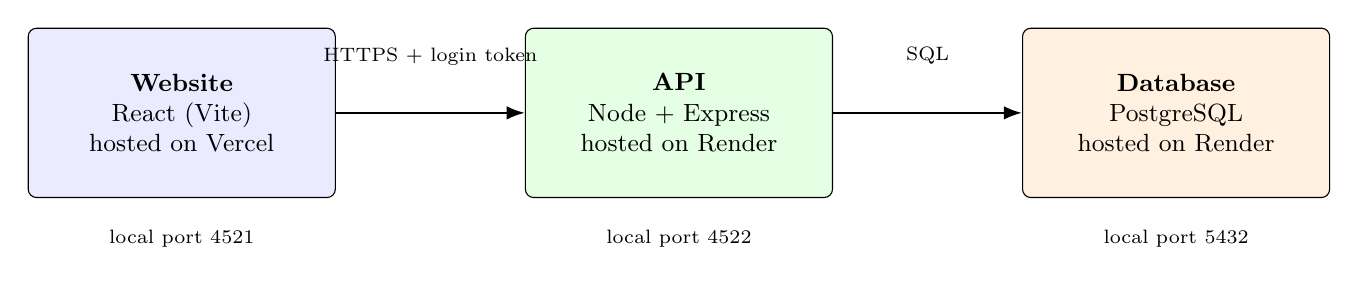
\begin{tikzpicture}[
  font=\small,
  box/.style={draw, rounded corners=3pt, align=center, inner sep=9pt,
              minimum width=3.9cm, minimum height=2.15cm},
  arr/.style={-{Latex}, thick}
]
\node[box, fill=blue!8] (ui) {\textbf{Website}\\React (Vite)\\hosted on Vercel};
\node[box, fill=green!10, right=2.4cm of ui] (api) {\textbf{API}\\Node + Express\\hosted on Render};
\node[box, fill=orange!12, right=2.4cm of api] (db) {\textbf{Database}\\PostgreSQL\\hosted on Render};

\draw[arr] (ui.east) -- (api.west);
\draw[arr] (api.east) -- (db.west);

\node[font=\scriptsize, align=center] at ($(ui)!0.5!(api)+(0,0.72)$) {HTTPS + login token};
\node[font=\scriptsize, align=center] at ($(api)!0.5!(db)+(0,0.72)$) {SQL};

\node[font=\scriptsize, below=0.28cm of ui] {local port 4521};
\node[font=\scriptsize, below=0.28cm of api] {local port 4522};
\node[font=\scriptsize, below=0.28cm of db] {local port 5432};
\end{tikzpicture}
\end{center}

On my laptop, the website uses \texttt{/api} and Vite sends that to the API. On the internet, the website uses\\
\url{https://kristball-giat.onrender.com/api}.

\subsection{What happens on one request}

\begin{enumerate}
  \item The API checks safety headers and who may call it.
  \item It writes a short access line (path and status only --- not the password).
  \item It checks the login token.
  \item It checks the role (admin / commander / logistics).
  \item If the person is not admin, it locks them to their own base.
  \item Then the real work runs (dashboard, purchase, transfer, and so on).
\end{enumerate}

Health checks skip the log, so the free ``keep awake'' ping does not fill the table.

\subsection{Tools used}

\begin{center}
\begin{tabular}{ll}
\toprule
\textbf{Part} & \textbf{Tool} \\
\midrule
Website & React, Vite, Tailwind, Axios, Chart.js, Recharts \\
API & Node.js, Express, TypeScript \\
Database & PostgreSQL + Prisma \\
Login & JWT token + bcrypt password hash \\
Local database & Docker \\
Live site & Vercel (website), Render (API + database) \\
API tests & Postman file in \texttt{postman/} \\
\bottomrule
\end{tabular}
\end{center}

\subsection{Folders}

\begin{lstlisting}
kristallball/
  backend/     API and database schema
  frontend/    website screens
  docs/        this report and schema.sql
  postman/     API tests
  docker-compose.yml
\end{lstlisting}

\section{How the numbers are counted}

Pick a start date and an end date.

\[
\text{Net movement} = \text{Purchases} + \text{Transfers in} - \text{Transfers out}
\]

\[
\text{Opening} = \text{(same net, assigned, expended) but only before the start date}
\]

\[
\text{Closing} = \text{Opening} + \text{Net movement} - \text{Assigned} - \text{Expended}
\]

Only transfers marked \textbf{Completed} count. A transfer that is still pending does not move stock yet.

For ``what is in the cage right now'':

\begin{itemize}
  \item Received = purchases + in $-$ out
  \item Still in store = received $-$ given to people
  \item Still with a person = given to them $-$ what they used
\end{itemize}

\textbf{Easy example.} PFC James Okonkwo got 10{,}000 bullets. He used 5{,}000 on the range. He still holds 5{,}000. Those used rounds do not go back on the shelf.

\section{Database picture}

We save events. We do not save a changing ``stock left'' field.

\subsection{Entity-relationship diagram}

Each arrow means ``this row points to that table''.

\begin{center}
\begin{tikzpicture}[
  font=\scriptsize,
  ent/.style={draw, align=center, inner sep=6pt,
              minimum width=3.35cm, minimum height=1.35cm}
]
\matrix (m) [
  matrix of nodes,
  nodes=ent,
  column sep=1.15cm,
  row sep=1.55cm
] {
  |(base)| {\textbf{Base}\\id, name, code, location}
    & |(eq)| {\textbf{Equipment type}\\category, name, unit}
    & |[draw=none,minimum width=3.35cm]| \\
  |(user)| {\textbf{User}\\username, role, base}
    & |(per)| {\textbf{Personnel}\\rank, service number}
    & |[draw=none,minimum width=3.35cm]| \\
  |(pur)| {\textbf{Purchase}\\qty, cost, date}
    & |(tr)| {\textbf{Transfer}\\from, to, qty, status}
    & |(asg)| {\textbf{Assignment}\\qty, date} \\
  |(aud)| {\textbf{Audit log}\\action, details}
    & |(http)| {\textbf{Access log}\\method, path, status}
    & |(ex)| {\textbf{Expenditure}\\qty, date} \\
};

\draw[-{Latex}] (user) -- (base);
\draw[-{Latex}] (per) -- (base);
\draw[-{Latex}] (pur) -- (base);
\draw[-{Latex}] (asg) -- (base);
\draw[-{Latex}] (tr) -- (base);
\draw[-{Latex}] (pur) -- (eq);
\draw[-{Latex}] (tr) -- (eq);
\draw[-{Latex}] (asg) -- (eq);
\draw[-{Latex}] (asg) -- (per);
\draw[-{Latex}] (ex) -- (asg);
\draw[-{Latex}] (aud) -- (user);
\draw[-{Latex}] (http) -- (user);
\end{tikzpicture}
\end{center}

A transfer has \textbf{two} bases: the one that sends, and the one that receives. Both point to Base.

\subsection{How tables link}

\begin{center}
\begin{tabular}{lll}
\toprule
\textbf{Table} & \textbf{Links to} & \textbf{Meaning} \\
\midrule
User & Base (optional) & Login person. Admin has no base. \\
Personnel & Base & Soldier who can hold gear (not a login). \\
Purchase & Base, Equipment type, User & New stock arrived. \\
Transfer & From base, To base, Equipment type, User & Stock moved. \\
Assignment & Base, Personnel, Equipment type, User & Gear given to a soldier. \\
Expenditure & Assignment, User & That soldier used some of it. \\
Audit log & User & What they changed. \\
Access log & User (optional) & Which page of the API was hit. \\
\bottomrule
\end{tabular}
\end{center}

\subsection{Main fields}

\begin{lstlisting}
Role: ADMIN | BASE_COMMANDER | LOGISTICS_OFFICER
Type: WEAPON | VEHICLE | AMMUNITION
Transfer status: PENDING | IN_TRANSIT | COMPLETED

bases, users, equipment_types, personnel
purchases, transfers, assignments, expenditures
audit_logs, api_access_logs
\end{lstlisting}

IDs are UUIDs. Fast-search indexes sit on base, equipment type, dates, and transfer status. Full SQL is in \texttt{docs/schema.sql}.

Why PostgreSQL (SQL), not a NoSQL store: purchases, transfers, and issues must all succeed together or not at all. SQL gives us that. Foreign keys stop a transfer to a base that does not exist. We can add up stock with normal sums. That matches ``count movements, not a cached number''.

When two people try to send the same stock at once, the database locks that base + item, counts again, then saves --- or it says no and undoes the whole step.

\section{Who can do what}

After login, the token holds \texttt{userId}, \texttt{role}, and \texttt{baseId}.

A commander or logistics officer cannot pick another base by editing the request. The server always uses the base on their token.

\begin{center}
\small
\begin{tabular}{>{\raggedright\arraybackslash}p{4.6cm}ccc}
\toprule
\textbf{Action} & \textbf{Admin} & \textbf{Commander} & \textbf{Logistics} \\
\midrule
See dashboard numbers & All bases & Own base & Own base \\
See stock and people & All bases & Own base & Own base (read) \\
Add a purchase & Yes & No & Own base \\
Send a transfer & Any base & No & From own base \\
Give gear to a soldier & Yes & Own base & No \\
Record used stock & Yes & Own base & No \\
See full history (Journal) & Yes & No & No \\
\bottomrule
\end{tabular}
\end{center}

The website hides buttons the same way. Journal is admin only. Purchase and transfer forms are for admin and logistics. Issue forms are for admin and commander.

\section{API list}

Most routes need the login token. Filters: start date, end date, base (admin only), equipment type.

\begin{center}
\small
\begin{longtable}{llp{6.8cm}}
\toprule
\textbf{Method} & \textbf{Path} & \textbf{What it does} \\
\midrule
\endfirsthead
\toprule
\textbf{Method} & \textbf{Path} & \textbf{What it does} \\
\midrule
\endhead
GET & \texttt{/api/health} & Public. Says the API is up. \\
POST & \texttt{/api/auth/login} & Public. Returns the token. \\
GET & \texttt{/api/auth/me} & Who is logged in. \\
GET & \texttt{/api/bases} & List of bases. \\
GET & \texttt{/api/equipment-types} & List of item types. \\
GET & \texttt{/api/personnel} & Soldiers. Own base if not admin. \\
GET & \texttt{/api/dashboard/summary} & Opening, net, closing. \\
GET & \texttt{/api/dashboard/holdings} & What is in the store. \\
GET & \texttt{/api/dashboard/personnel-holdings} & What each person still holds. \\
GET & \texttt{/api/dashboard/net-movement} & Detail for the pop-up. \\
GET / POST & \texttt{/api/purchases} & List / add stock. Write: admin or logistics. \\
GET / POST & \texttt{/api/transfers} & List / send stock. Completed transfers check quantity. \\
PATCH & \texttt{/api/transfers/:id/status} & Pending $\rightarrow$ in transit $\rightarrow$ completed. \\
GET / POST & \texttt{/api/assignments} & List / give gear. Write: admin or commander. \\
GET / POST & \texttt{/api/assignments/expenditures} & List / record used stock. Cannot use more than remaining. \\
GET & \texttt{/api/audit-logs} & Admin change history. \\
GET & \texttt{/api/audit-logs/access} & Admin API hit history. \\
\bottomrule
\end{longtable}
\end{center}

Login body:

\begin{lstlisting}
POST /api/auth/login
{ "username": "admin_user", "password": "AdminPass123!" }
\end{lstlisting}

There are two logs on purpose:

\begin{itemize}
  \item \textbf{Audit log} --- saved with the change. If the change is undone, this line is undone too.
  \item \textbf{Access log} --- saved after the reply. Path and status only. Passwords are never stored.
\end{itemize}

\section{Website screens}

\begin{center}
\begin{tabular}{llp{7.4cm}}
\toprule
\textbf{Screen} & \textbf{Link} & \textbf{What you see} \\
\midrule
Login & \texttt{/login} & Name and password. \\
Sitrep & \texttt{/} & Three big numbers, filters, stock table, chart. Click net movement for the break-down. \\
Inbound & \texttt{/purchases} & Add new stock (if allowed). History with date and equipment filters. \\
Cross-level & \texttt{/transfers} & Send stock to another base. \\
Issue & \texttt{/assignments} & Give gear to a soldier. Record what they used. \\
Journal & \texttt{/audit} & Admin history. \\
\bottomrule
\end{tabular}
\end{center}

\section{How to run it on a laptop}

Need Node 20+, npm, Git, and Docker.

\begin{lstlisting}
git clone https://github.com/tsj2003/kristball.git
cd kristball

cp .env.example .env
cp .env.example backend/.env
cp frontend/.env.example frontend/.env
# put a long JWT_SECRET in .env and backend/.env

docker compose up -d
npm install
npm run db:setup
npm run dev
\end{lstlisting}

Then open \url{http://localhost:4521}. API check: \url{http://localhost:4522/api/health}.

Import the Postman file. Run ``Login as admin'' first.

\begin{center}
\begin{tabular}{ll}
\toprule
\textbf{Setting} & \textbf{Meaning} \\
\midrule
\texttt{DATABASE\_URL} & How to reach Postgres \\
\texttt{JWT\_SECRET} & Secret used to sign the login token \\
\texttt{JWT\_EXPIRES\_IN} & How long the token lasts (\texttt{8h}) \\
\texttt{PORT} & API port \\
\texttt{CORS\_ORIGIN} & Which website may call the API \\
\texttt{VITE\_API\_BASE\_URL} & Website's API address \\
\bottomrule
\end{tabular}
\end{center}

\section{How it is hosted}

\begin{center}
\begin{tabular}{ll}
\toprule
\textbf{Part} & \textbf{Link} \\
\midrule
Website & \url{\livefront} \\
API & \url{\liveapi} \\
Code & \url{\livegit} \\
\bottomrule
\end{tabular}
\end{center}

Render build:

\begin{lstlisting}
npm install --include=dev && npx prisma generate --schema=backend/prisma/schema.prisma && npm run build -w backend
\end{lstlisting}

Render start:

\begin{lstlisting}
npx prisma migrate deploy --schema=backend/prisma/schema.prisma && npm run start -w backend
\end{lstlisting}

Demo users were loaded \textbf{once}. Seed is not left in the start command, so a restart does not wipe data.

The website is allowed to call the API (\texttt{CORS\_ORIGIN} is the Vercel link). Render free sleeps after about 15 minutes. UptimeRobot opens \texttt{/api/health} every 5 minutes so the demo stays up.

\section{Test logins}

These work on the live site.

\begin{center}
\begin{tabular}{llll}
\toprule
\textbf{Role} & \textbf{Username} & \textbf{Password} & \textbf{Base} \\
\midrule
Admin & \texttt{admin\_user} & \texttt{AdminPass123!} & All bases \\
Base commander & \texttt{commander\_alpha} & \texttt{CommandPass123!} & Fort Alpha \\
Logistics officer & \texttt{logistics\_officer} & \texttt{LogisticsPass123!} & Fort Alpha \\
\bottomrule
\end{tabular}
\end{center}

Names on screen: Col.\ Hannah Reeves (admin), LTC David Okoye (commander), MAJ Sofia Alvarez (logistics).

Demo data in short:

\begin{itemize}
  \item Three bases: Fort Alpha, Fort Bravo, Station Charlie.
  \item Humvees, trucks, M4s, AK-47s, 5.56 and 9\,mm ammo.
  \item Stock was bought, then some was sent to other bases.
  \item PFC James Okonkwo got 10{,}000 rounds and used 5{,}000. He still has 5{,}000.
\end{itemize}

On the live home page (1 Jan 2026 to 17 Sep 2026, all bases): opening 0, net movement 125{,}057, expended 5{,}000, closing 110{,}048.

\section{What the brief asked for}

Every point below is in the code, in this report, and on the live site.

\begin{center}
\small
\begin{tabular}{>{\raggedright\arraybackslash}p{5.6cm}p{8.6cm}}
\toprule
\textbf{Ask} & \textbf{Where it is} \\
\midrule
Opening, closing, net movement (purchases + in $-$ out), assigned, expended & Home page cards. Formula in section 3. File \texttt{backend/src/services/inventory.ts}. \\
Filters: date, base, equipment type & Home page. Admin can pick base. Others stay on their base. \\
Click net movement $\rightarrow$ purchases / in / out pop-up & Click the yellow net card. File \texttt{NetMovementModal.tsx}. \\
Record purchases for a base & Inbound page. Logistics + admin. \\
Purchase history with date and equipment filters & Inbound page filters. API: \texttt{GET /api/purchases}. \\
Transfers between bases + history with time and item & Cross-level page. Status and timestamps in the table. \\
Assign to personnel + expended & Issue page. \\
Admin sees all; commander own base; logistics purchases and transfers & Section 5. Middleware \texttt{auth.ts}. Website hides the wrong forms. \\
React, responsive, easy to move around & Vite + Tailwind. Menu is a row on a phone and a side list on a computer. \\
Secure REST API + JWT roles in middleware & Express routes. Helmet, CORS, \texttt{authenticateToken}, \texttt{authorizeRoles}, \texttt{enforceBaseScope}. \\
Log all purchases, transfers, assignments & \texttt{AuditLog} with the save. \texttt{ApiAccessLog} for every API call. \\
SQL database that can track movements & PostgreSQL. Events, not a cached stock field. \\
Stock cannot go below zero & Transfer and issue check available qty. HTTP 409 if not enough. \\
Demo logins work on the live site & Section 11. Website \url{\livefront}. \\
\texttt{/login} works on Vercel & \texttt{frontend/vercel.json} sends all paths to the app. \\
Render stays awake & UptimeRobot hits \texttt{/api/health} every 5 minutes. \\
\bottomrule
\end{tabular}
\end{center}

\section{What I turn in}

\begin{center}
\begin{tabular}{ll}
\toprule
\textbf{Item} & \textbf{Where} \\
\midrule
This PDF & compiled from \texttt{docs/Kristallball-Report.tex} \\
Code zip & \texttt{npm run pack:submission} \\
Schema & \texttt{docs/schema.sql} \\
Postman & \texttt{postman/Kristallball.postman\_collection.json} \\
Live website & \url{\livefront} \\
Live API & \url{\liveapi/api/health} \\
\bottomrule
\end{tabular}
\end{center}

\section{Why I built it this way}

\begin{enumerate}
  \item Count from real events, do not store a number that can go stale.
  \item Save a transfer as one all-or-nothing step, so stock cannot go below zero.
  \item Let a transfer sit as pending until it is really done.
  \item Keep change history with the change. Keep API hits in a second table, with no passwords.
  \item Trust the login token for ``which base'', not whatever the browser sends.
\end{enumerate}

\vspace{1em}
\noindent\textit{End of report.}

\end{document}
